\section{System Overview}

Pixels is an adaptive storage system on top of HDFS.
As shown in Figure~\ref{fig:overview}, it contains six functional modules:
\begin{itemize}
	\item \textit{Data Ingestion}. Unlike traditional ETL process on HDFS in which data is transformed into specific format in a batch manner, in Pixels, data is ingested into the system in a streaming manner.
	We assume that the analytical workload mostly accesses the most recent data, so that we do not reload the historical data.
	When the Layout generator generates a new data layout, it is only applied on the new coming data.
	
	\item \textit{Workload Modeling}. Workload modeling is responsible for collecting the query workload and build workload models. Access patterns (columns accessed by queries) and filters (predicates) of the queries are collected by this module.
	Then the access patterns and filters are used to build a workload model by which we can predict the access patterns and filters in the coming future. In pixels, we use hidden Markov chain to model the workload.
	
	\item \textit{Layout Generator}. Layout generator optimizes the data layout with the workload model built by \textit{Workload Modeling} module and the reading cost model built by \textit{Reading Cost Modeling}.
	Data layout optimization is triggered by workload modeling module when the workload model is significantly changed.
	The new data layout generated and evaluated by layout generator is then provided to \textit{Data Ingestion} module to be applied in the new coming data.
	
	\item \textit{Data Split Generator}. Each data reading task reads a data split.
	Traditionally, each mapper task reads a HDFS block as a data split by default, while in Pixels, the data split is adaptively generated by data split generator, which takes both of task execution parallelism and HDFS block size into consideration.

	\item \textit{Column Chunk Caching}. Column chunk caching is a local cache manager for column chunks in Pixels files. 
	Compared with HDFS block as the default cache unit, column chunk is a much smaller storage unit, and can improve cache hitting rate greatly.
	
	\item \textit{Reading Cost Modeling}. Reading cost modeling moudle collects and maintains disk reading costs, which are used to build the data reading cost model.
	The model is sent to \textit{Layout Generator} for layout optimization.
	Data statistics are also collected and maintained and used by \textit{Data Split Generator} to optimize data splits of reading tasks and used by \textit{Data Ingestion} module to optimize data encoding and indexing.
\end{itemize}

\begin{figure}[h!]
	\vspace{-1em}
	\centering
	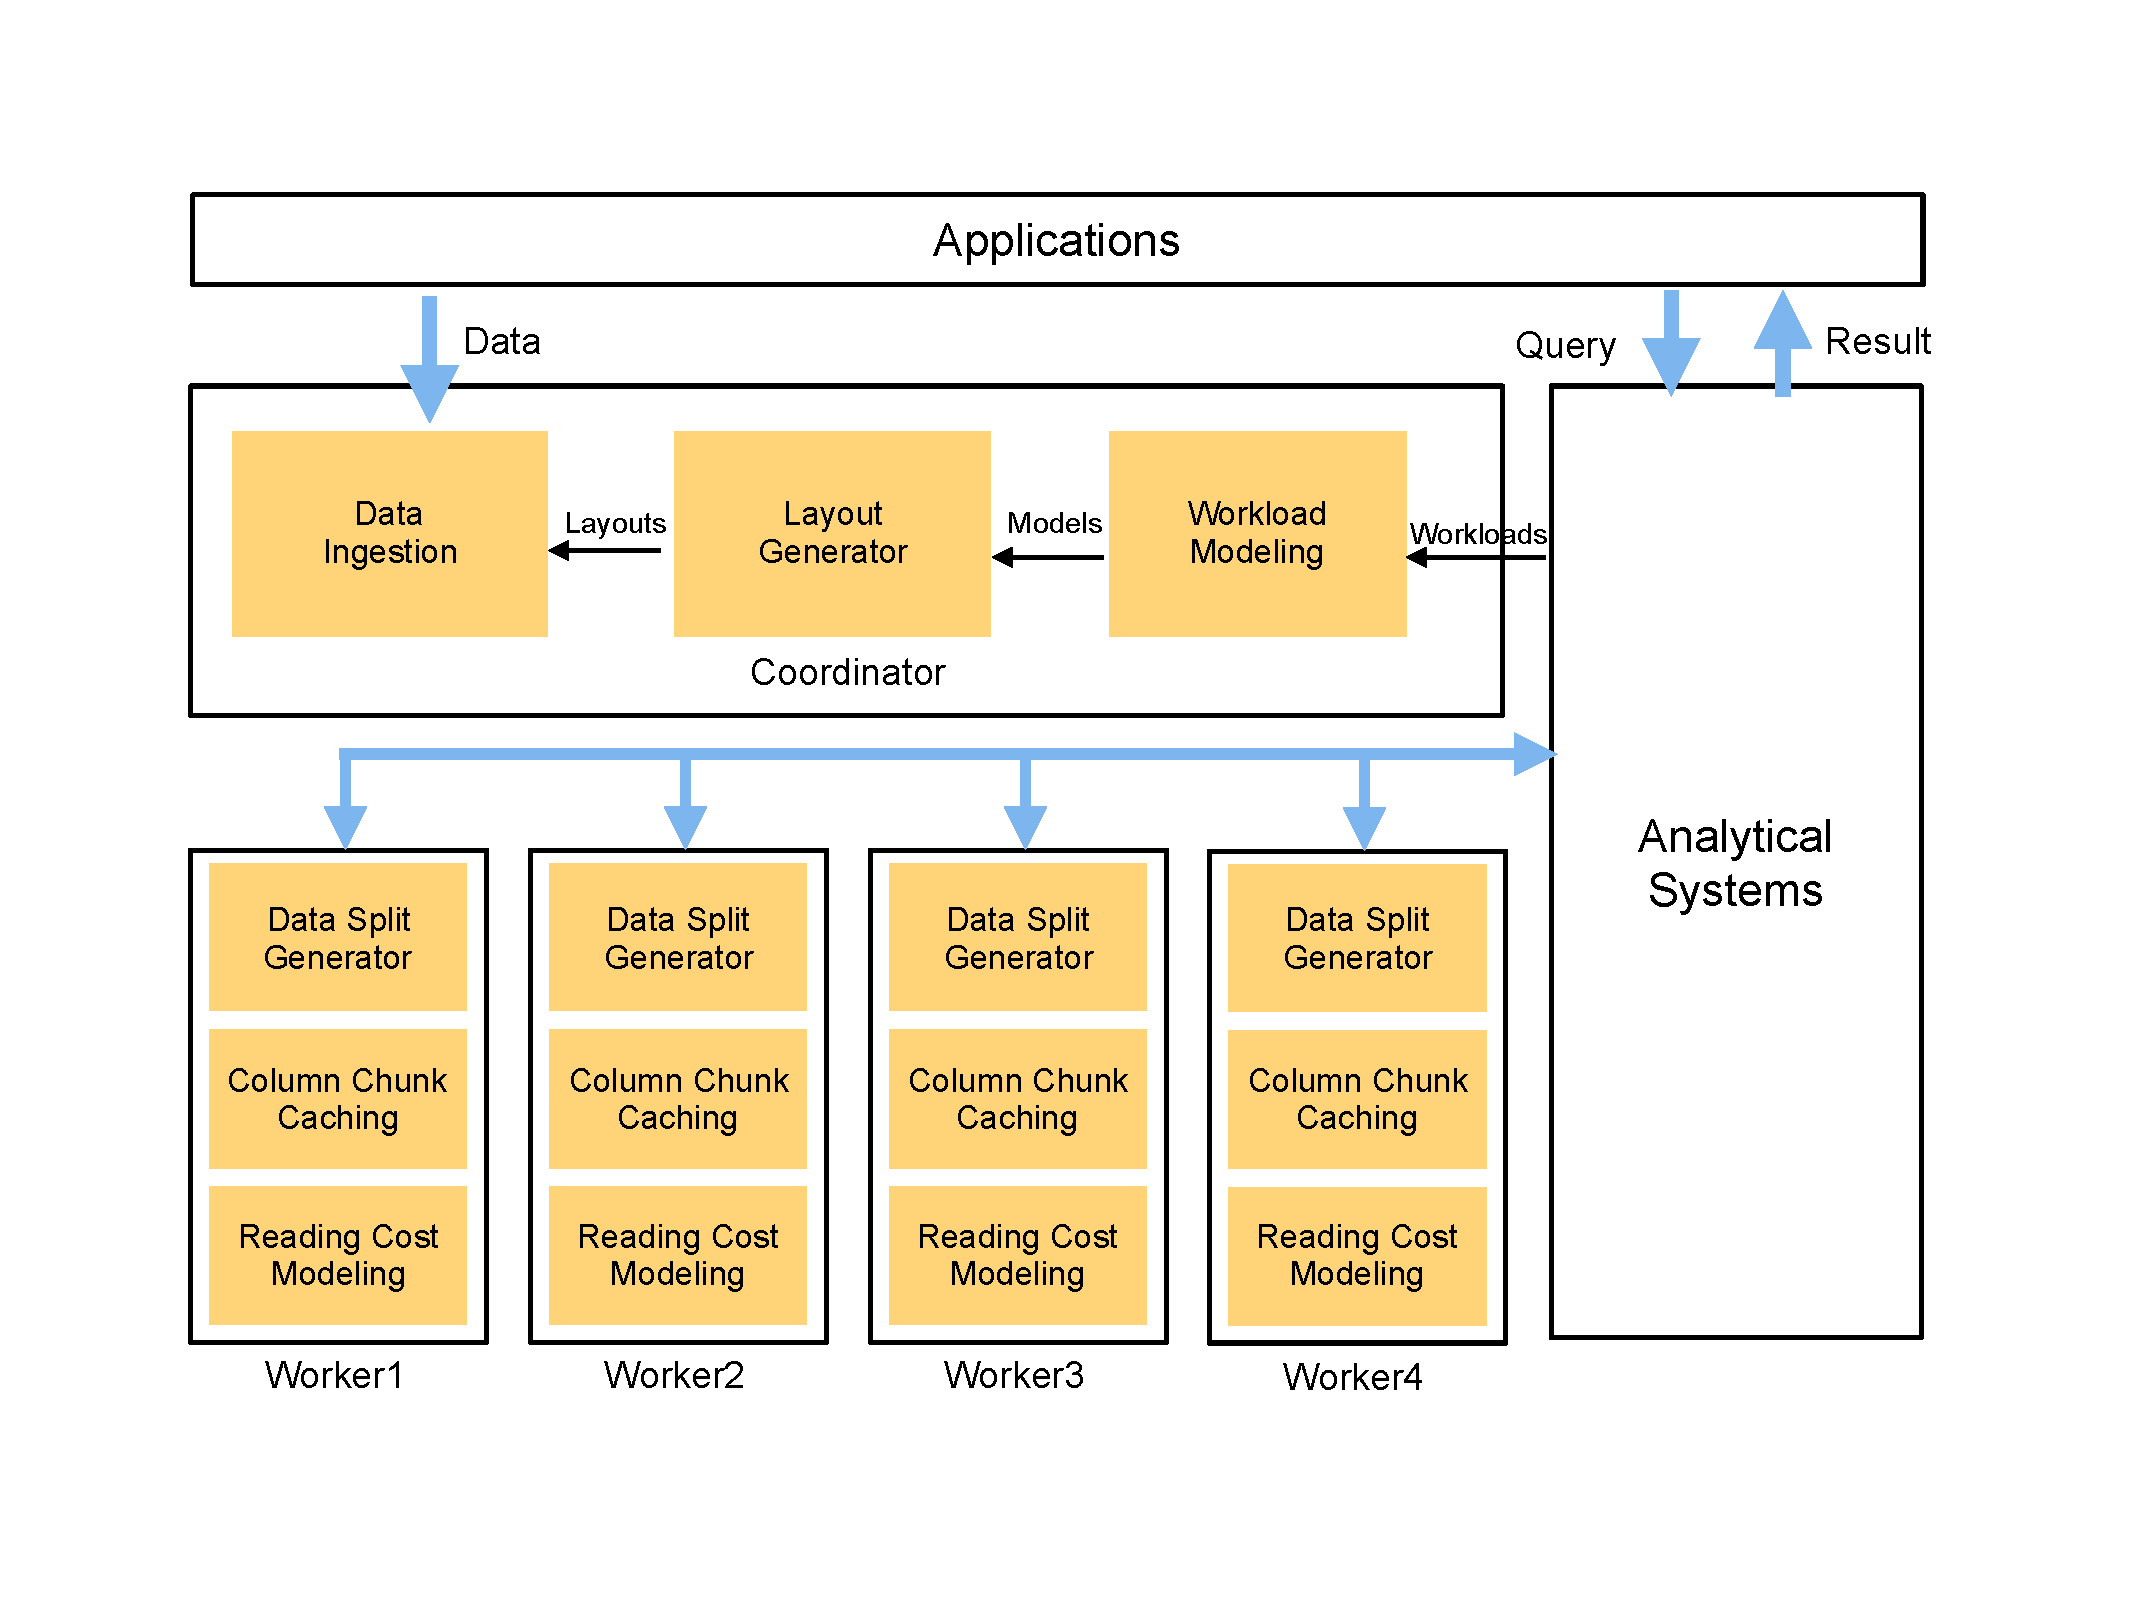
\includegraphics[width=0.5\textwidth, height=0.36\textwidth]{figs/framework}
	\vspace{-3em}
	\caption{System Framework of Pixels}\label{fig:overview}
	\vspace{-0em}
\end{figure}

As a whole system, \textit{Workload Modeling}, \textit{Layout Generator} and \textit{Data Ingestion} modules are located on \textit{Coordinator} node in the cluster. \textit{Data Split Generator}, \textit{Column Chunk Caching} and \textit{Reading Cost Modeling} modules are resided on each worker node.

User data are ingested by data ingestion module in a streaming manner.
Meanwhile, queries are submitted to analytical systems, e.g. Spark SQL, Presto, and query workloads are collected by workload modeling module.
Upon significant change of workload model, layout generator module optimizes data layout based on new workload model and then generates a new data layout, which is applied in data ingestion module in the new coming data.
During query execution, analytical systems get the data split strategy through data split generator module, and then data reading tasks access column chunks through column chunk caching module.
When cache missing happens, column chunk caching module is responsible for reading column chunks from disk into caching buffer. During cache accessing and disk reading, reading cost modeling module collects and maintains data statistics and disk reading costs.
